\chapter{Implementasi}

\section{Detail Implementasi}

Seluruh komponen dibuat dengan menggunakan bahasa python. Kakas dibuat dengan bentuk library python
sehingga dapat diinstall dengan mudah menggunakan \emph{pip}. Kakas didesain untuk menguji
program yang juga ditulis dengan bahasa python. Kode implementasi dan pengujian terdapat
di repositori \\\url{https://gitlab.informatika.org/rid9/thesis}.

\subsection{Parser}

Komponen \emph{parser} berfungsi untuk membaca \emph{file} fitur dan menguraikan isinya menjadi
struktur data yang dapat diolah. Komponen ini hanya menghasilkan skenario dalam bentuk dasar
yang hanya berisi step-step, sehingga semua bentuk skenario yang lebih kompleks
seperti \emph{scenario outline} akan diuraikan terlebih dahulu menjadi semua kemungkinan
kombinasi skenario dasarnya. Sebagai contohnya adalah

\begin{lstlisting}[language=gherkin]
Scenario Outline: menambahkan barang ke dalam keranjang
  Given user <login state> login
  When user memasukkan 1 barang
  Then <result state> ada 1 barang di dalam keranjang
  Examples:
    | login state | result state |
    | sudah       | sukses       |
    | belum       | gagal        |
\end{lstlisting}

Kode diatas akan diuraikan menjadi skenario dasar dengan bentuk

\begin{lstlisting}[language=gherkin]
Scenario: menambahkan barang ke dalam keranjang (1)
  Given user sudah login
  When user memasukkan 1 barang
  Then sukses ada 1 barang di dalam keranjang
Scenario: menambahkan barang ke dalam keranjang (2)
  Given user belum login
  When user memasukkan 1 barang
  Then gagal ada 1 barang di dalam keranjang
\end{lstlisting}

Perubahan ini berfungsi agar komponen \emph{runtime} hanya perlu tahu cara menjalankan
skenario dasar saja sehingga lebih simpel, dan juga memperbanyak jumlah step yang diketahui
oleh kakas sehingga dapat membangkitkan skenario acak yang lebih beragam.

Kode penguraian menggunakan arsitektur \emph{Parsing Expression Grammar} (PEG), dimana
pada arsitektur ini setiap \emph{non-terminal} seperti \texttt{scenario, scenarioOutline, feature}
yang ada dalam \emph{grammar} pada \ref{sec:struktur-bahasa} dibentuk menjadi fungsi-fungsi
yang dapat disusun, sehingga kode penguraian mirip dengan \emph{grammar}. Fungsi-fungsi
ini memiliki tipe parameter dan kembalian yang sama sehingga
dapat dikomposisikan menghasilkan fungsi yang lebih kompleks. Pada psudeocode dibawah
akan diilustrasikan kode penguraian untuk grammar \texttt{scenario} simpel.

\begin{lstlisting}[language=python]
# fungsi kombinator
def optional(func)      # func?
def zero_or_more(func)  # func*
def one_or_more(func)   # func+
def or(func1, func2,..) # func1 | func2 | ..
def literal(string)     # "string"
def parseString(input)  # string
def newline(input):
  return literal("\n")(input)

def parseStepKeyword:
  return or(literal("given"), literal("when"), literal("then"))

def parseStepLine(input):
  keyword, input = parseStepKeyword(input)
  line, input = parseString(input)
  _, input = newline(input)
  return Step(keyword, line), input

def parseScenarioKeyword:
  return or(
    literal("scenario"),
    literal("fail scenario")
  )

def parseStepLines(input):
  return one_or_more(parseStepLine)(input)

def parseScenario(input):
  keyword, input = parseScenarioKeyword(input)
  _, input = literal(":")(input)
  desc, input = parseString(input)
  _, input = newline(input)
  steps, input = parseStepLines(input)

  return Scenario(keyword, desc, steps), input
\end{lstlisting}


\subsection{Importer}

Importer berfungsi untuk membaca \emph{file} step descriptor yang ditulis dalam python.
Importer menghasilkan kumpulan fungsi \emph{step descriptor} yang akan digunakan untuk
menjalankan step-step yang telah didefinisikan dari skenario.

Importer akan membaca semua file python yang ada dalam folder fitur, lalu mencoba untuk
mencari semua fungsi yang merupakan step descriptor yang memiliki \emph{decorator} python.
Semua fungsi ini lalu dikumpulkan dan diteruskan ke komponen \emph{runtime}.
Cara kerja importer secara simpel digambarkan oleh \emph{psudeocode} berikut:

\begin{lstlisting}[language=python]
def feature_folder
def step_descriptors = []

for file in feature_folder:
  file_objects = import(file)
  for function in file_objects.functions:
    if function is step descriptor:
      step_descriptors.add(function)

return step_descriptors
\end{lstlisting}

\subsubsection{API}

Komponen ini adalah bagian dari kakas \emph{library} yang digunakan oleh user untuk menulis
\emph{step descriptor}. Bagian ini meng-\emph{export} decorator-decorator yang disediakan.
Decorator ini berfungsi untuk menandai fungsi sebagai \emph{step descriptor} sehingga dapat
dibedakan dari fungsi biasa oleh \emph{importer}. Cara kerja descriptor dan contoh penggunaannya
digambarkan oleh \emph{psudeocode} berikut:

\begin{lstlisting}[language=python]
def step_decorator(keyword, function):
  mark function as step decorator
  return function
def given(func):
  return step_decorator("given", func)
def when(func):
  return step_decorator("when", func)
def then(func):
  return step_decorator("then", func)

# contoh penggunaan
@given("user awalnya punya {num} kue")
def step1(num):
  user.kue = num

@when("user memakan {num} kue")
def step2(num):
  user.kue -= num

@then("user sisa kue {num}")
def step3(num):
  assert user.kue == num
\end{lstlisting}


\subsection{Runtime}

Runtime berfungsi untuk menjalankan pengujian. Runtime menerima hasil dari parser dan importer,
mencocokkan step-step dalam skenario dengan fungsi \emph{step descriptor} yang cocok,
dan kemudian menjalankan skenario pengujian.

Runtime menghasilkan laporan penjalanan pengujian. Laporan ini berisi skenario apa saja
yang berhasil dan gagal. Laporan ini juga berisi penyebab kegagalan skenario dalam
bentuk catatan exception.

Bagian runtime juga berfungsi untuk membangkitkan skenario acak dari \emph{step} yang telah ada
dan menjalankannya.




\section{Validasi}

Pada tugas akhir ini akan digunakan kosa kata validasi untuk membedakan pengujian yang dilakukan oleh kakas ini terhadap program user (pengujian)
dengan pengujian yang dilakukan terhadap kakas ini (validasi).

\subsection{Tujuan Validasi}

Validasi dilakukan dengan tujuan untuk mengevaluasi apakah kakas yang dibuat dapat digunakan dengan
baik dan membantu programmer untuk menemukan kelemahan keamanan pada perangkat lunak.
Dalam validasi juga ditentukan apakah kakas yang dibuat mudah digunakan atau masih ada kekurangan.

\subsection{Skenario Validasi}

Validasi dilakukan dengan cara membuat file fitur untuk suatu proyek tertentu secara perlahan hingga semua fitur
telah diuji secara BDD. Proyek yang akan diuji adalah proyek sistem perwalian mahasiswa dimana terdapat data mahasiswa, ipk,
serta sks yang akan diambil. Sistem memiliki business logic dimana sks hanya bisa diambil menurut ipk, jika ipk kurang sama dari
2 maka mahasiswa tidak dapat mengambil lebih dari 20 sks. Sistem juga akan mengecek bahwa mahasiswa tidak bisa disetujui
jika belum melakukan pembayaran.

Validasi dimulai dengan membuat proyek kosong python. Kemudian dilanjutkan dengan menulis \emph{file feature}
dengan satu skenario. Kemudian \emph{step definition} dibuat untuk semua step yang dibuat. Setelah \emph{file}
pengujian dibuat dilanjutkan dengan membuat program yang mengimplementasikan skenario tersebut. Jika semua
test untuk skenario telah berjalan dengan baik, dibuat \emph{file feature} untuk skenario selanjutnya.
Dalam pengerjaan juga dilakukan \emph{refactor} dengan fitur yang telah didesain.

\subsection{Hasil Validasi}

Berikut adalah kode gherkin yang digunakan untuk validasi program.

\begin{lstlisting}[language=gherkin]
Variable:
    paid status: enum true, false
    approve status: enum true, false

Feature: mahasiswa feature
    Scenario: create mahasiswa default
        Given prepare mahasiswa 001
        When create mahasiswa 001
        Then mahasiswa 001 exists
    
    Fail Scenario: create mahasiswa fail
        Given prepare mahasiswa 002
        When create mahasiswa 001
        Then mahasiswa 003 exists

    Scenario Outline: sks must correct for approve
        Given prepare mahasiswa 001
        Given mahasiswa 001 have paid true
        Given mahasiswa 001 ipk is <ipk>
        Given mahasiswa 001 ambil sks <sks>
        Given mahasiswa 001 approve <approve>
        When create mahasiswa 001
        Then mahasiswa 001 exists

        Example:
            | ipk   | sks   | approve   |
            | 4     | 24    | true      |
            | 2     | 20    | true      |
            # bisa tidak approve walaupun sks benar
            | 4     | 24    | false     |

        Fail Example:
            | ipk   | sks   | approve   |
            | 2     | 24    | true      |


    Scenario: must have paid before approve
        Given prepare mahasiswa 001
        Given mahasiswa 001 have paid <paid status>
        Given mahasiswa 001 approve <approve status>
        When create mahasiswa 001
        Then mahasiswa 001 exists

        Variable Rejected:
            | paid status  | approve status  |
            | false        | true            |


    Scenario Outline: ipk range
        Given prepare mahasiswa 001
        Given mahasiswa 001 ipk is <ipk>
        When create mahasiswa 001
        Then mahasiswa 001 exists
        Example:
            | ipk   |
            | 0     |
            | 2     |
            | 4     |
        Fail Example:
            | ipk  |
            | -1.0 |
            | 5.0  |

    
    Scenario Outline: sks range
        Given prepare mahasiswa 001
        Given mahasiswa 001 ipk is 4
        Given mahasiswa 001 ambil sks <sks>
        When create mahasiswa 001
        Then mahasiswa 001 exists

        Example:
            | sks   |
            | 0     |
            | 12    |
            | 24    |
        Fail Example:
            | sks   |
            | -1    |
            | 25    |
    
    Scenario Outline: batas ambil sks menurut ipk
        Given prepare mahasiswa 001
        Given mahasiswa 001 ipk is <ipk>
        Given mahasiswa 001 ambil sks <sks>
        When create mahasiswa 001
        Then mahasiswa 001 exists
        Example:
            | ipk   | sks   |
            | 4     | 24    |
            | 4     | 12    |
            | 4     | 0     |
            | 2     | 20    |
        Fail Example:
            | ipk   | sks   |
            | 2     | 24    |
            | 2     | 21    |
\end{lstlisting}

Dan berikut adalah hasil dari eksekusi validasi.

% \begin{figure}[h]
%   \centering
%   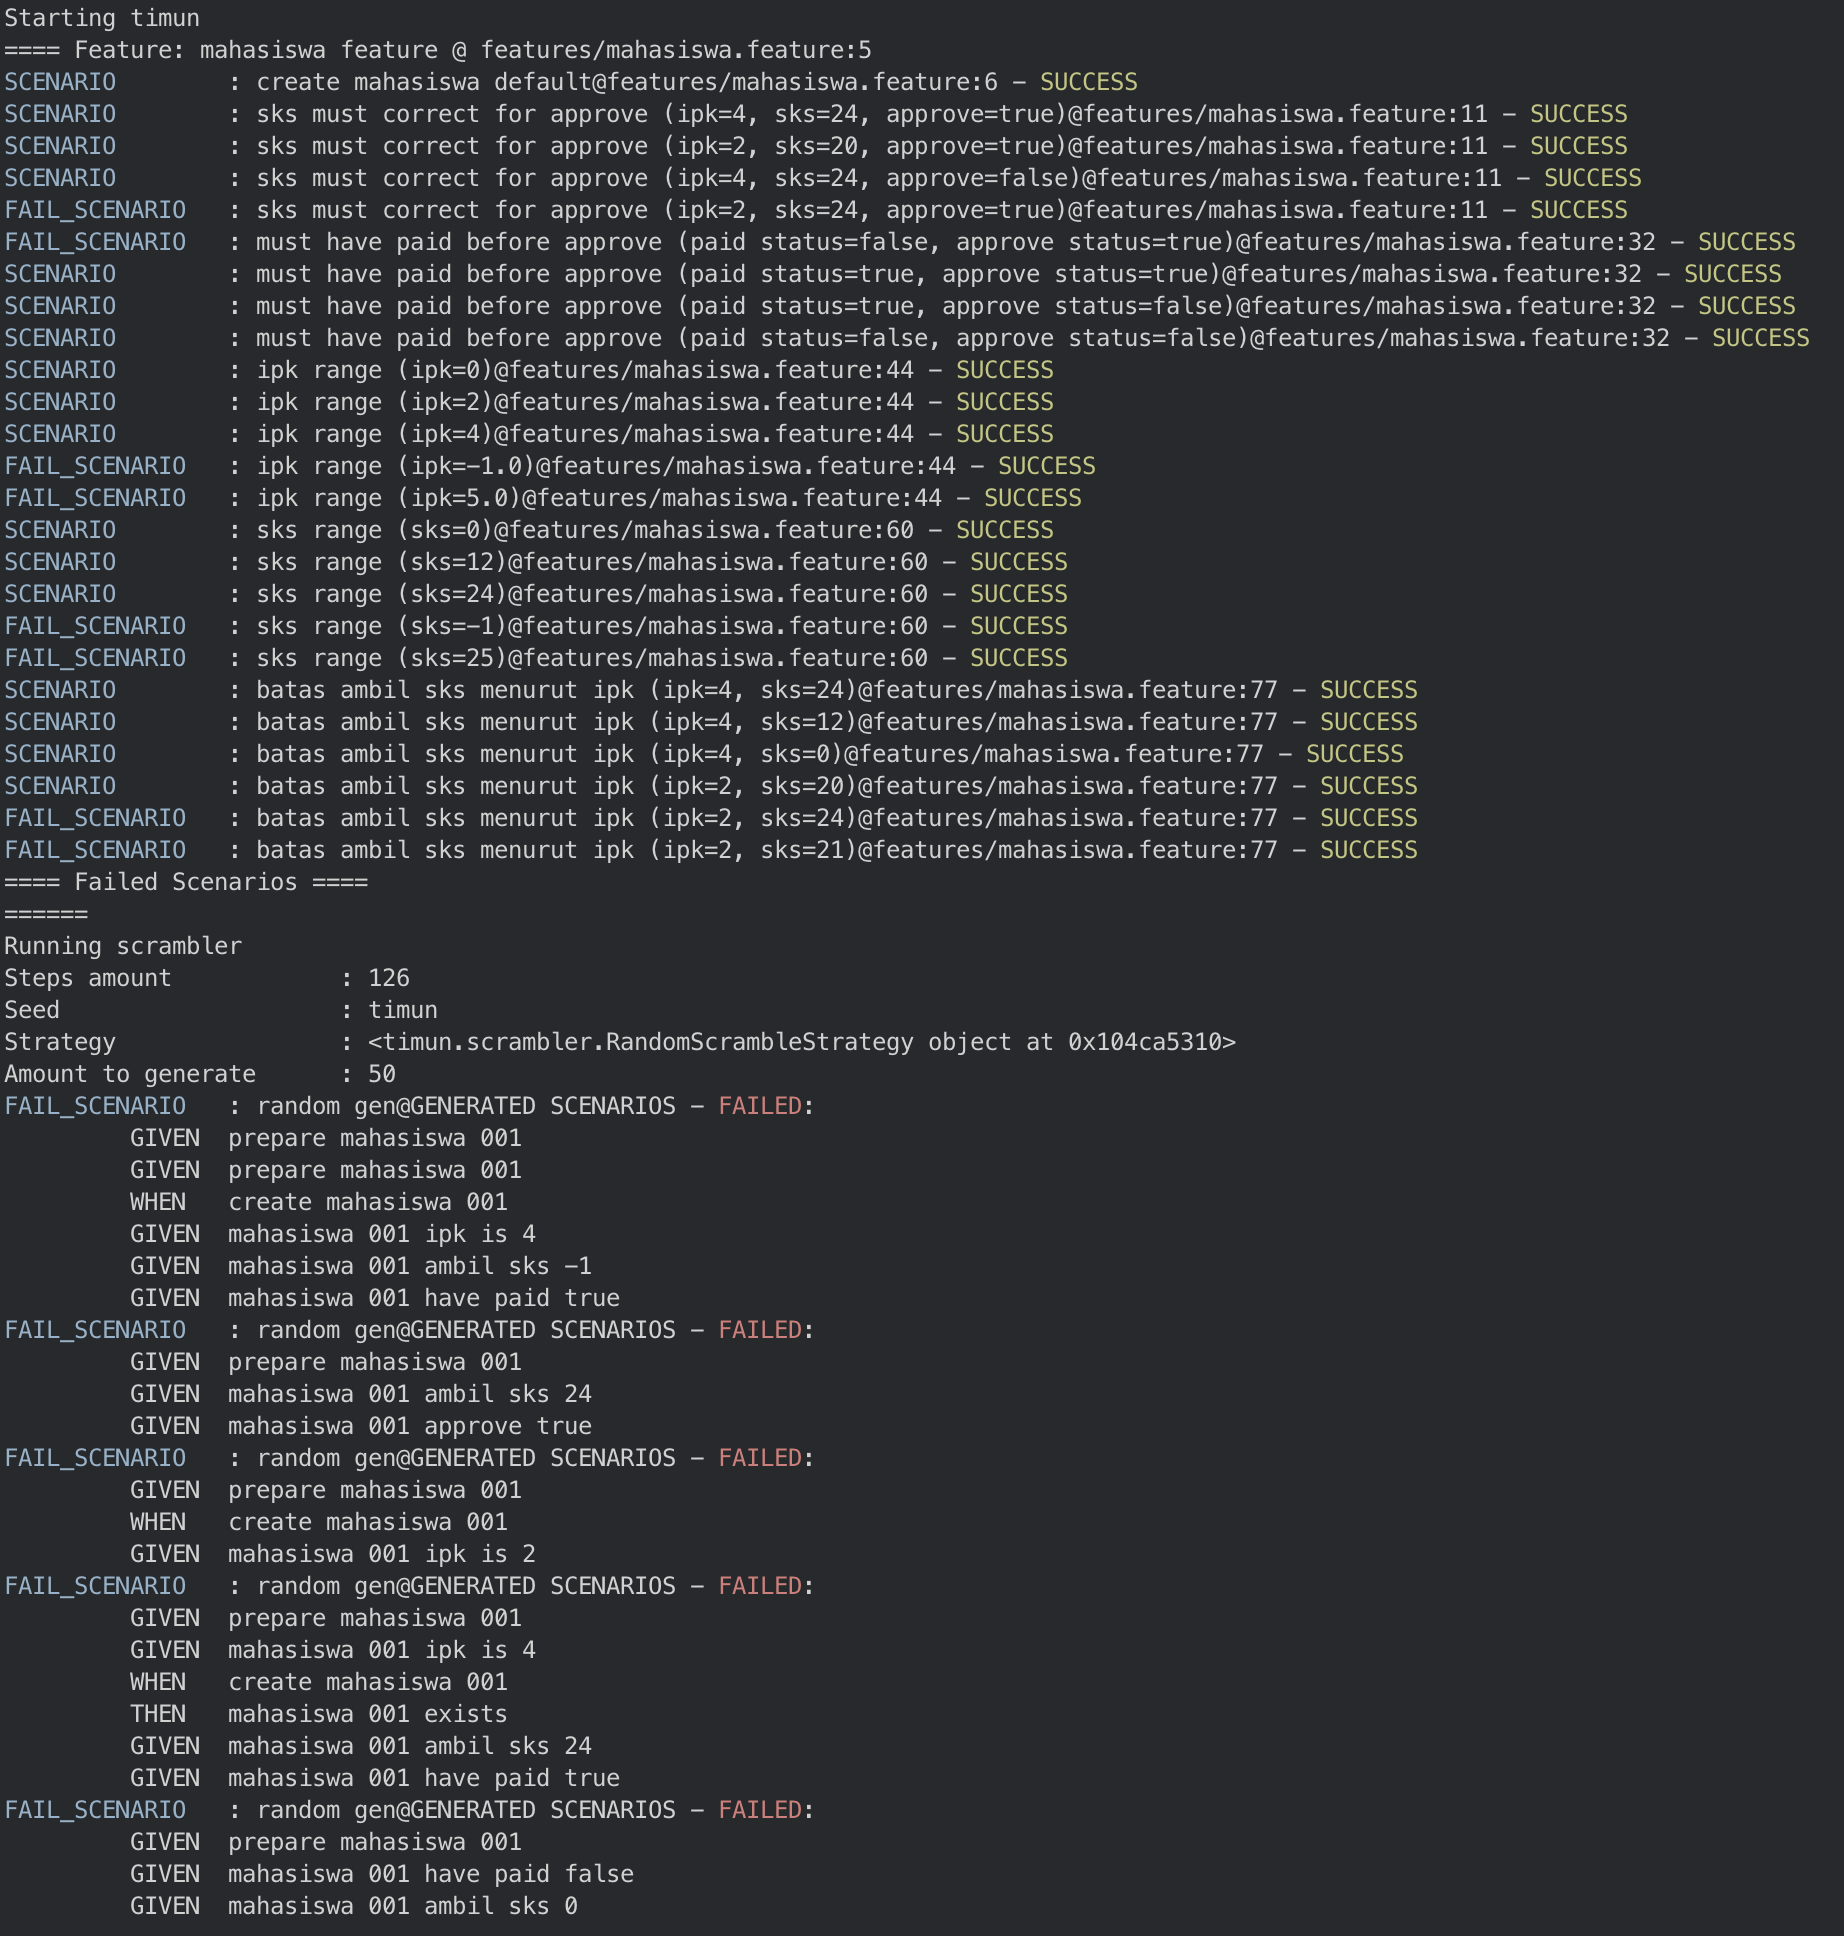
\includegraphics[width=0.8\textwidth]{resources/result.png}
%   \caption{Hasil Pengujian}
%   \label{dia:test-result}
% \end{figure}
\begin{lstlisting}[language=testresult]
Starting timun
==== Feature: mahasiswa feature @ features/mahasiswa.feature:5
SCENARIO	: create mahasiswa default@features/mahasiswa.feature:6 - SUCCESS
FAIL_SCENARIO	: create mahasiswa fail@features/mahasiswa.feature:11 - SUCCESS
SCENARIO	: sks must correct for approve (ipk=4, sks=24, approve=true)@features/mahasiswa.feature:16 - SUCCESS
SCENARIO	: sks must correct for approve (ipk=2, sks=20, approve=true)@features/mahasiswa.feature:16 - SUCCESS
SCENARIO	: sks must correct for approve (ipk=4, sks=24, approve=false)@features/mahasiswa.feature:16 - SUCCESS
FAIL_SCENARIO	: sks must correct for approve (ipk=2, sks=24, approve=true)@features/mahasiswa.feature:16 - SUCCESS
FAIL_SCENARIO	: must have paid before approve (paid status=false, approve status=true)@features/mahasiswa.feature:37 - SUCCESS
SCENARIO	: must have paid before approve (paid status=true, approve status=true)@features/mahasiswa.feature:37 - SUCCESS
SCENARIO	: must have paid before approve (paid status=true, approve status=false)@features/mahasiswa.feature:37 - SUCCESS
SCENARIO	: must have paid before approve (paid status=false, approve status=false)@features/mahasiswa.feature:37 - SUCCESS
SCENARIO	: ipk range (ipk=0)@features/mahasiswa.feature:49 - SUCCESS
SCENARIO	: ipk range (ipk=2)@features/mahasiswa.feature:49 - SUCCESS
SCENARIO	: ipk range (ipk=4)@features/mahasiswa.feature:49 - SUCCESS
FAIL_SCENARIO	: ipk range (ipk=-1.0)@features/mahasiswa.feature:49 - SUCCESS
FAIL_SCENARIO	: ipk range (ipk=5.0)@features/mahasiswa.feature:49 - SUCCESS
SCENARIO	: sks range (sks=0)@features/mahasiswa.feature:65 - SUCCESS
SCENARIO	: sks range (sks=12)@features/mahasiswa.feature:65 - SUCCESS
SCENARIO	: sks range (sks=24)@features/mahasiswa.feature:65 - SUCCESS
FAIL_SCENARIO	: sks range (sks=-1)@features/mahasiswa.feature:65 - SUCCESS
FAIL_SCENARIO	: sks range (sks=25)@features/mahasiswa.feature:65 - SUCCESS
SCENARIO	: batas ambil sks menurut ipk (ipk=4, sks=24)@features/mahasiswa.feature:82 - SUCCESS
SCENARIO	: batas ambil sks menurut ipk (ipk=4, sks=12)@features/mahasiswa.feature:82 - SUCCESS
SCENARIO	: batas ambil sks menurut ipk (ipk=4, sks=0)@features/mahasiswa.feature:82 - SUCCESS
SCENARIO	: batas ambil sks menurut ipk (ipk=2, sks=20)@features/mahasiswa.feature:82 - SUCCESS
FAIL_SCENARIO	: batas ambil sks menurut ipk (ipk=2, sks=24)@features/mahasiswa.feature:82 - SUCCESS
FAIL_SCENARIO	: batas ambil sks menurut ipk (ipk=2, sks=21)@features/mahasiswa.feature:82 - SUCCESS
==== Failed Scenarios ====
======
Running scrambler
Steps amount		: 129
Seed			: .
Strategy		: <timun.scrambler.RandomScrambleStrategy object at 0x10897d2e0>
Amount to generate	: 50
FAIL_SCENARIO	: random gen@GENERATED SCENARIOS - FAILED:
	 GIVEN	prepare mahasiswa 001
	 GIVEN	mahasiswa 001 ambil sks -1
	 GIVEN	mahasiswa 001 ambil sks 20
	 WHEN	create mahasiswa 001
	 THEN	mahasiswa 001 exists
	 GIVEN	prepare mahasiswa 001
FAIL_SCENARIO	: random gen@GENERATED SCENARIOS - FAILED:
	 GIVEN	prepare mahasiswa 001
	 WHEN	create mahasiswa 001
	 THEN	mahasiswa 001 exists
FAIL_SCENARIO	: random gen@GENERATED SCENARIOS - FAILED:
	 GIVEN	prepare mahasiswa 001
	 GIVEN	prepare mahasiswa 001
	 WHEN	create mahasiswa 001
	 GIVEN	mahasiswa 001 approve false
	 THEN	mahasiswa 001 exists
\end{lstlisting}


\subsection{Analisa Hasil Validasi}

Pada paparan hasil validasi diatas, fitur representasi kegagalan ditampilkan pada kode baris 11-14,
32-43, 59-62, 77-80, 94-97 dan hasil eksekusinya terdapat pada hasil baris 4, 16-17, 21-22, 27-28.
Fitur kemampuan menyatakan variansi ditampikan pada kode baris 1-3 dan 37-46, sementara hasil eksekusi
terdapat pada hasil baris 9-12.

Fitur pengacakan skenario ditampilkan pada hasil baris 31-52. Dapat dilihat bahwa dari 50 skenario yang dibangkitkan,
terdapat 3 skenario yang tidak lulus (skenario yang dibangkitkan seharusnya gagal saat dijalankan namun skenario ini tidak gagal).
Ada beberapa penyebab skenario ini tidak lulus.
Pertama kakas pembangkitan menghasilkan skenario yang telah dinyatakan benar pada kode gherkin sehingga menghasilkan \textit{false negative}.
Kedua kakas pembangkitan menghasilkan skenario dengan alur logika yang tidak berurut (given-when-then), pada beberapa \textit{seed}
lain kakas juga tidak menghasilkan skenario yang memiliki step \texttt{then} sehingga tidak ada pengecekan yang dilakukan.
Dari beberapa seed yang digunakan, kakas masih belum menghasilkan skenario acak yang menemukan kesalahan logika pada program,
hal ini dapat terjadi karena ukuran program pengujian yang tidak terlalu besar menyebabkan implementasi yang tidak memiliki kelemahan,
kurang banyaknya skenario yang dibangkitkan, atau karena pembangkitan skenario yang belum terlalu efektif.

Pada proses pembuatan kode gherkin, ditemukan kekurangan terhadap rancangan dimana fitur-fitur yang dirancang
tidak dapat berkerjasama dengan baik dalam keadaan tertentu. Fitur ini adalah \emph{fail example} dengan \emph{variable rejecte}
dimana jika digunakan bersamaan akan menghasilkan \emph{double negative} yang menyebabkan skenario pengujian lebih
sulit untuk dipahami dan tidak berjalan sesuai ekspektasi.

Untuk kemudahan, melalui studi lain \cite{dsl_lesson} ditemukan bahwa penggunaan DLS BDD seperti Gherkin walaupun
pada awalnya terlihat menjanjikan namun dalam waktu lama dibutuhkan standarisasi bahasa yang digunakan, karena tiap
orang yang menulis kasus pengujian dapat mendeskripsikan kasus dengan cara yang berbeda-beda. \emph{User} yang
akan menggunakan kakas pengujian juga memerlukan pelatihan dalam penggunaan kerangka pikir dan kakas untuk menghasilkan
kasus pengujian yang baik.

% Dari hasil diatas dapat dilihat bahwa fitur pengujian biasa seperti fitur dari gherkin,
% representasi kegagalan, dan deklarasi variabel telah bejalan dengan baik.
% Fitur-fitur ini membantu penulis untuk menemukan kekurangan dalam pengujian ataupun implementasi selama
% penulisan.
% Namun selama
% pengembangan kakas ditemukan bahwa fitur deklarasi variabel tidak dapat berkerja sama dengan
% fitur representasi kegagalan menggunakan \texttt{Fail Example Scenario Outline}, dimana
% saat menggunakan deklarasi variabel dengan tabel \texttt{Variable Rejected} dan tabel \texttt{Fail Example}
% terjadi negatif ganda dan sulit untuk dimengerti. Hal ini menyebabkan fitur tabel \texttt{Variable} tidak dapat
% digunakan besamaan dengan fitur \texttt{Scenario Outline}.

% Untuk fitur pengacakan skenario masih banyak menghasilkan false positive dan false negative karena
% pembangkitan skenario acak yang masih sangat simpel dan belum mengikuti urutan yang seharusnya.